%% 2/18/2016
%%%%%%%%%%%%%%%%%%%%%%%%%%%%%%%%%%%%%%%%%%%%%%%%%%%%%%%%%%%%%%%%%%%%%%%%%%%%
% AGUJournalSample.tex: this sample file is for articles formatted with LaTeX
%
% This sample file includes commands and instructions
% given in the order necessary to produce a final output that will
% satisfy AGU requirements.
%
% PLEASE DO NOT USE YOUR OWN MACROS
% DO NOT USE \newcommand, \renewcommand, or \def.
%
% FOR FIGURES, DO NOT USE \psfrag or \subfigure.
% DO NOT USE \psfrag or \subfigure commands.
%
%%%%%%%%%%%%%%%%%%%%%%%%%%%%%%%%%%%%%%%%%%%%%%%%%%%%%%%%%%%%%%%%%%%%%%%%%%%%
%
% Step 1: Set the \documentclass
%
% There are two options for article format:
%
% 1) PLEASE USE THE DRAFT OPTION TO SUBMIT YOUR PAPERS.
% The draft option produces double spaced output.
% 
% 2) numberline will give you line numbers.

% Tip:
%  To add line numbers to lines in equations:
%  \begin{linenomath*}
%  \begin{equation}
%  \end{equation}
%  \end{linenomath*}

%% To submit your paper:
\documentclass[linenumbers,draft]{agujournal}

% Now, type in the journal name: \journalname{<Journal Name>}
% ie,
\journalname{Geophysical Research Letters}

%% Choose from this list of Journals:
%
% JGR-Atmospheres
% JGR-Biogeosciences
% JGR-Earth Surface
% JGR-Oceans
% JGR-Planets
% JGR-Solid Earth
% JGR-Space Physics
% Global Biochemical Cycles
% Geophysical Research Letters
% Paleoceanography
% Radio Science
% Reviews of Geophysics
% Tectonics
% Space Weather
% Water Resource Research
% Geochemistry, Geophysics, Geosystems
% Journal of Advances in Modeling Earth Systems (JAMES)
% Earth's Future
% Earth and Space Science


%% ------------------------------------------------------------------------ %%
%
%  ENTER Title Page commands:
%
%% ------------------------------------------------------------------------ %%

% (A title should be specific, informative, and brief. Use
% abbreviations only if they are defined in the abstract. Titles that
% start with general terms then specific results are optimized in
% searches)

% Example: \title{This is a test title}

% (List authors by first name or initial followed by last name and
% separated by commas. Use \affil{} to number affiliations, and
% \thanks{} for author notes.  
% Additional author notes should be indicated with \thanks{} (for
% example, for current addresses). 

% Example: \authors{A. B. Author\affil{1}\thanks{Current address, Antartica}, B. C. Author\affil{2,3}, and D. E.
% Author\affil{3,4}\thanks{Also funded by Monsanto.}}

% (include name and email addresses of the corresponding author.  More
% than one corresponding author is allowed in this LaTeX file and for
% publication; but only one corresponding author is allowed in our
% editorial system.)  

%% Corresponding Author:
% Corresponding author mailing address and e-mail address:

% Example: \correspondingauthor{First and Last Name}{email@address.edu}

% Authors are individuals who have significantly contributed to the
% research and preparation of the article. Group authors are allowed, if
% each author in the group is separately identified in an appendix.)

% \affiliation{1}{First Affiliation}
% \affiliation{2}{Second Affiliation}
% \affiliation{3}{Third Affiliation}
% \affiliation{4}{Fourth Affiliation}

%% Keypoints, final entry on title page.
% Example: 
% \begin{keypoints}
% \item	List up to three key points (at least one is required)
% \item	Key Points summarize the main points and conclusions of the article
% \item	Each must be 100 characters or less with no special
% characters or punctuation 
% \end{keypoints}

%% \begin{abstract} begins second page 

%%%%%%%%%%%%%%%%%%%%%%%%%%%%%%%%%%%%%%%%%%%%%%%%%%%%%%%%%%%%%%%%%%%%%
% Track Changes:
% To add words, \added{<word added>}
% To delete words, \deleted{<word deleted>}
% To replace words, \replace{<word to be replaced>}{<replacement word>}
% To explain why change was made: \explain{<explanation>}

% At the end of the document, use \listofchanges, which will list the
% changes and the page and line number where the change was made.

% When final version, \listofchanges will not produce anything,
% \added{} word will be printed, \deleted{} will take away the word,
% \replaced{}{} will print only the 2nd argument.
% \explain will not print anything.

% Optional argument:
% You can also add additional information to be printed with the list
% of changes, to indicate the initials of the person changing the text,
% and the time and/or date of the change, or any other comment by using
% the optional [] argument:
% \added[AH, 3:30pm, Feb 18, 2016]{added term}
% will yield 
% [AH, 3:30pm, Feb 18, 2016] added term on page...
%%%%%%%%%%%%%%%%%%%%%%%%%%%%%%%%%%%%%%%%%%%%%%%%%%%%%%%%%%%%%%%%%%%%%
\usepackage{amsmath,amssymb}
\usepackage{siunitx}
\usepackage{graphicx}

\begin{document}

%% ------------------------------------------------------------------------ %%
%
%  TITLE
%
%% ------------------------------------------------------------------------ %%


\title{Quantifying the effect of channelization of pyroclastic density currents from multiphase modeling }


%% ------------------------------------------------------------------------ %%
%
%  AUTHORS AND AFFILIATIONS
%
%% ------------------------------------------------------------------------ %%

 \authors{Allison Kubo \affil{1}
Josef Dufek \affil{1}}

\affiliation{1}{Department of Earth Sciences, University of Oregon, Eugene, Oregon, USA.}


%% Corresponding Author
%(include name and email addresses of the corresponding author.  More
%than one corresponding author is allowed in this Word file and for
%publication; but only one corresponding author is allowed in our
%editorial system.)  

\correspondingauthor{Allison Kubo}{akubo@uoregon.edu}

%  List up to three key points (at least one is required)
%  Key Points summarize the main points and conclusions of the article
%  Each must be 100 characters or less with no special characters or punctuation 

\begin{keypoints}
\item Runout distance in increased in channelized flows 
\item Entrainment of ambient gas is decreased
\item Channelization increases turbulence
\end{keypoints}

%% ------------------------------------------------------------------------ %%
%
%  ABSTRACT
%
%% ------------------------------------------------------------------------ %%


\begin{abstract}

Due to their mobility and high velocities, pyroclastic density currents (PDCs) represent a major hazard around many volcanoes. These the buoyancy, fluidization, and stratification of these particle-laden gravity currents is controlled by the entrainment of ambient air. From field studies, it is clear that topography can play a role in the amount of entrainment. We present three-dimensional multiphase models of channelized PDCs and link the entrainment to channel geometry (width, depth, sinuosity, and slope). Our simulations span the range of natural channels found in volcanic landforms and show that channelization increases run out distances. We also explore the conditions necessary for channel overspill. 

\end{abstract}

%% ------------------------------------------------------------------------ %%
%
%  TEXT
%
%% ------------------------------------------------------------------------ %%

%%% Suggested section heads:
% \section{Introduction}
% 
% The main text should start with an introduction. Except for short
% manuscripts (such as comments and replies), the text should be divided
% into sections, each with its own heading. 

% Headings should be sentence fragments and do not begin with a
% lowercase letter or number. Examples of good headings are:

% \section{Materials and Methods}
% Here is text on Materials and Methods.

% \subsection{A descriptive heading about methods}
% More about Methods.
% 
% \section{Data} (Or section title might be a descriptive heading about data)
% 
% \section{Results} (Or section title might be a descriptive heading about the
% results)
% 
% \section{Conclusions}


\section{Introduction}
\label{sec:intro}
Pyroclastic density currents (PDCs) are highly mobile particle-laden gravity currents. Due to their ability to subsume terrain obstacles and their large runout distances, PDCs are one of the most dangerous of eruptive products (Auker, 2013). PDCs span a range of particle concentrations not only between events but spatially and temporarily within the current ( Sparks, 1976; Druitt, 1998). They are roughly separated into three regimes. The majority of the current visible to human is the dilute clouds where dynamics are controlled by gas entrainment and buoyancy. As particles fall out of the billowing dilute portion, they form a suspended load or bed-load (Dufek and Bergantz, 2006). At the base, particle-particle interactions dominate and there is relatively low permeability. Dense portions of the current can become mobile due to self fluidization when the pore pressure supports the dense matrix (Wilson, 1980; Roche, 2012; Breard et al., 2018). 

The entrainment of ambient air controls the buoyancy, fluidization, and mobility of these currents (Ellison and Turner 1959; Sparks, 1976; Bursik and Woods, 1996;  Branney and Kokelaar, 2002; Andrews, 2014). Entrainment of air occurs in two main mechanisms Kelvin-Helmholtz and Lobe-Cleft instabilities. Kelvin-Helmholtz instabilities occur due to shearing of dilute portions of the flow while Lobe-Cleft instabilities occur at the head of the flow where gas is entrained when the nose of the current hangs over the base of the current. Entrainment leads to thermal expansion of gas as it is heated by the erupted gas and particles which increases the height of the PDCs and will eventually lead to buoyancy reversal and lift off. Entrainment can also increase the pore fluid pressure in the flow. 

The entrainment into these flows is linked to the density stratification and the interaction with topography (Valentine, 1987; Andrews and Manga, 2011; Doronzo et al., 2011)). Dilute currents, thicker due to entrainment and thermal expansion, are able to surmount topography. In addition, decoupling of dense and dilute portions adds another factor of uncertainty in flow predictions (Fisher, 1995). Channelization of PDCs, in particular, has large effects on the runout distance and mobility of flows (Charbonnier and Gertisser, 2011; Komorowski, 2013; Brand et al., 2016). It is necessary to understand how channelization effects entrainment and stratification in these flows to understand runout distances and possible channel avulsion which presents both of which present large hazards to people living around PDC producing volcanoes.

In this work, we apply three-dimensional multiphase numerical models of PDCs over idealized topographies spanning natural terrains to develop a framework for understanding how channel geometry, sinuosity, and amplitude affect entrainment and avulsion of the current.  

\section{Case Study: Merapi 2010}
\label{sec:Case}
The Merapi 2010 dome collapse painfully illustrates the hazards due to PDCs complex interactions with topography. Located between the Central Java and Yogyakarta Provinces, Mount Merapi is infamous for producing silicic domes preceding PDC formation or following destructive explosions at the summit (Voight et al., 2000). In 1872, an explosion lasting 5 days destroyed of the summit and is associated with voluminous PDCs due to column collapse (Hartman,1932), however, the past 100 years have been characterized by VEI 1-3 eruptions. Dome collapses occur when they become unstable due to gravity or overpressured and often produce PDCs dubbed Merapi-type (Bardintzeff, 1984). The majority of eruptions in the 19th and 20th centuries have been oriented down the southwest flank of the volcano leading to increased settlement on the northwest flanks until 2010 when 1.3 million people living within a 20 km radius from the summit (Mei et al., 2015). Prior to 2010, channelized flows from Merapi had runout distances of 4-8 km depending on topography (Charbonnier and Gertisser, 2011, Charbonnier et al., 2013, ).

On 5 November 2010, after rapid dome inflation disintegration of the dome began a multistage eruption during the night. Of interest in this paper are Stages 4 and 5 which produced PDCs of 15.5 km run out distances. The paroxysmal dome collapse of Stage 4 produced high energy and velocity confined and unconfined PDCs. The high-energy events produced few fatalities due to evacuations however channelized flows between 10-15km from the summit caused ~ 170 fatalities (Komorowski et al., 2013).  The flows were able to subsume the 185 m Gendol Ridge near the summit resulting in detached dilute flows over the ridge and dense channelized flows in the Gendol valley. 

Four distinct PDCs made it into the Gendol Valley each of which spilled out of the channel with progressively longer runout distances (Lube, 2011; Komorowski et al., 2013, Gertisser et al., 2013). The overspill locations for the flows were all located at bends in the channel of various amplitude and wavelength. One jump location is associated with a Sabo dam, man-made channel confinement meant to reduce sediment flow in the river. Three of four of the flows overspill then become re-confined in the nearby Tlogo valley where there are secondary over banking events.  Analysis of the geometry of the channels by Lube (2011), shows that avulsion events are correlated to areas where the cross-sectional area of the channel decreases and where the sinuosity increases. Grain distribution of the overflow and the confined facies both show a similar bimodal distribution at 1 and 2 \(\phi\) indicates that the avulsion mechanism was the overflow of the basal region not a decoupling of the dilute portion. After overflowing, the dilute portions likely did decouple and form surge deposits that are found interbedded with the overflow deposits (Lube, 2011). 
\section{Methods}
\label{sec:meth}
\subsection{Topography Analysis}
Erosional channels on the slope of volcanoes are ubiquitous and the possible channel geometries are near infinite thus to narrow our parameter range we performed a statistical analysis on the channel forms seen on 5 different PDC producing volcanoes: Merapi, Monserrat, Unzen, Colima, and Sakurajima. These are by no means representative of all channels in volcanic landscapes but provide a basis for creating idealized terrains for the multiphase models. The parameters we will vary include: slope, channel wavelength, amplitude, depth, and width. 

For a first-order approach to this parameter space, the authors used Google Earth Pro to measure channel length, downvalley length, width and depth profiles, and measured the dominant wavelengths. The authors analyzed 25 channels in total and 184 transects across those channels for width and depth (See Appendix A1). 

Our analysis shows that channel depths are strongly associated with channel widths despite that they varied significantly from channel to channel and along their downstream length. Seventy percent of channels have an aspect ratio (W/D) of between 5 and 15. Although the average channel depth was 33.7 m the distribution shows that much deeper channels (+50m) while relatively less prominent were also observed. Deeper channels should also be modeled considering the incredible mobility of PDCs. 

\begin{figure}[h]
 \centering
 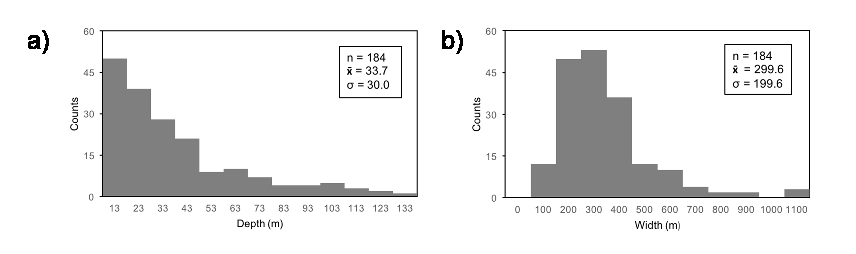
\includegraphics{dist.eps}
 \caption{ Analysis of 184 individual transects over 32 channels at our sampled volcanoes. \textbf{a)} Shows the distribution of channel depths most channels are between 10 and 30 m deep however the span of channel depths is wide. \textbf{b)} Shows the widths of channels, few channels are ls than 200 m wide and most are 300-500 m wide.}
 \label{fig:hist} 
\end{figure}

The channels exhibited sinuosities between 1.08 and 1.26 with an average of 1.13. There were no disernable trends between sinuosity and aspect ratio; there may be a minor positive correlation between sinuosity and average slope but more data would be necessary to confirm this. There is a clear corelation between wavelength and associated amplitude and generally the wavelength is 4-10 times the amplitude. Additionally, the highest observed wavelength also correlated positively with the largest wavelength where the largest is three times larger than the smallest. 
The averages slopes of the channels varied between 11 and 25 degrees with maximum slopes of over 60 degrees proximal to the summit. 

\begin{figure}[ht]
 \centering
 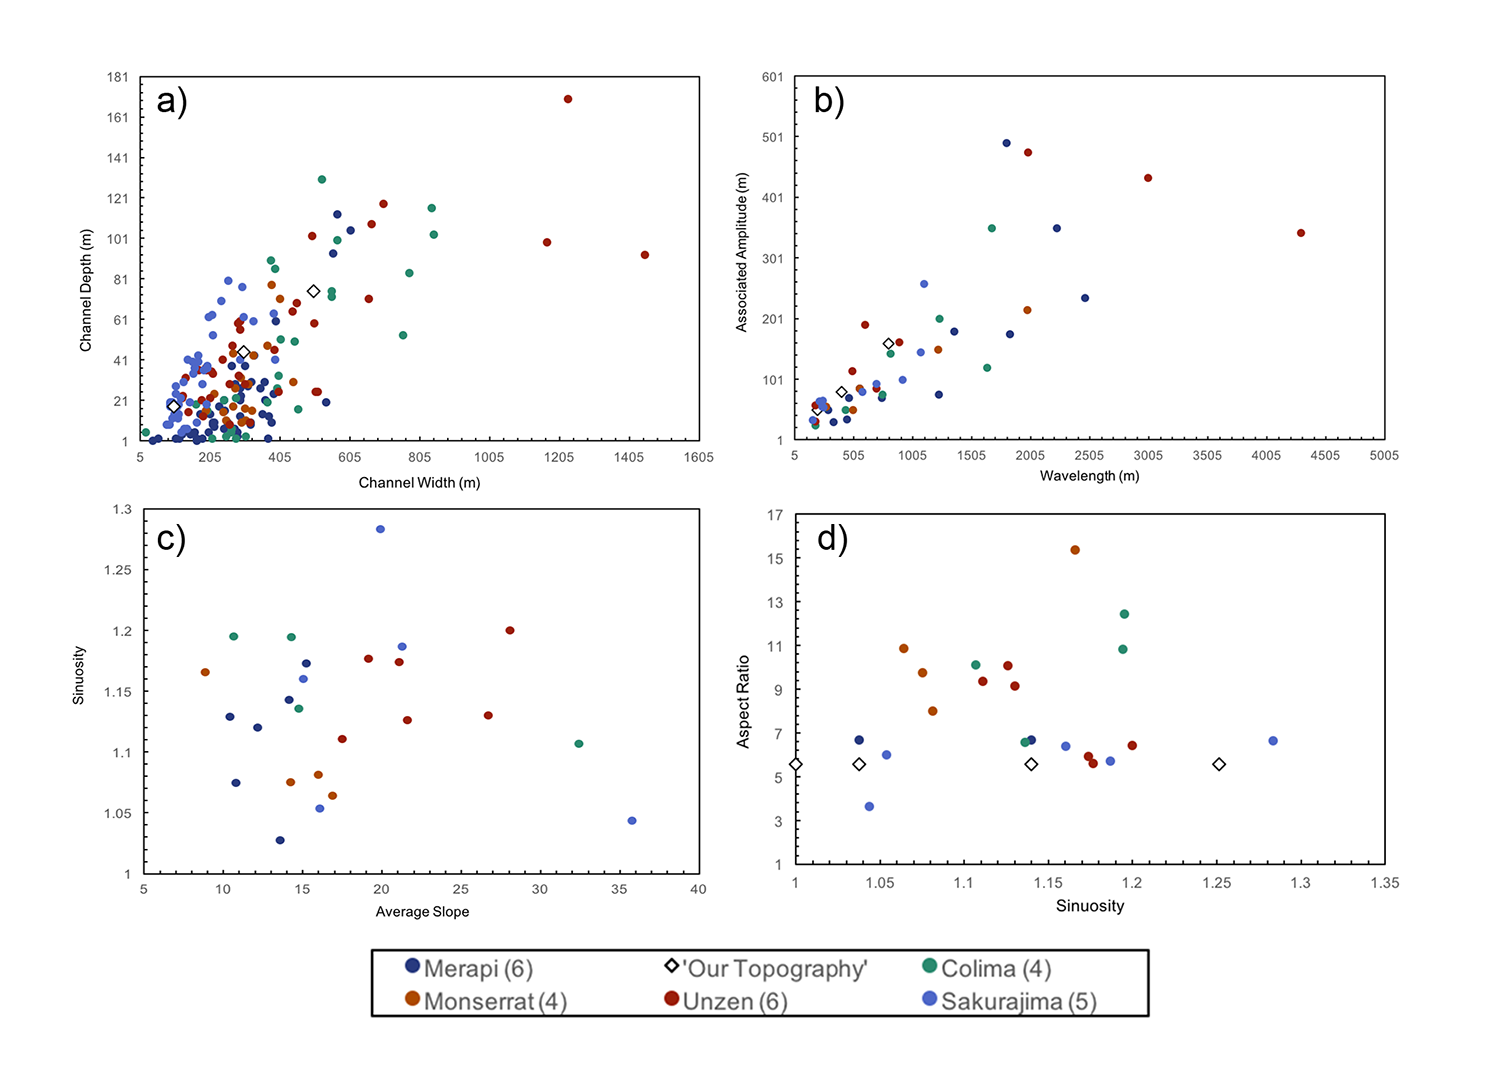
\includegraphics[width= \linewidth]{topography.png}
 \caption{ Trends seen in the 25 analyzed channels. Clear positive trends in \textbf{a)} and \text{b)} however any trends in \textbf{c)} and \textbf{d)} are unclear. The topography of our simulations spans the natural channels}
 \label{fig:topo} 
\end{figure}


\subsection{Multiphase Simulation}
Using the topography parameters from above, the authors have run 4** three-dimensional multiphase models which solve for two phases: a gas phase (water vapor) and a particle phase ( \(250 \mu m \), Stokes number \char`\~   \(  10^{-4}\)) at 2 m grid resolution. The model includes an equation for the mass (Eq. 1), momentum (Eq.2), and thermal conservation (Eq.3) for both the particle phase and the gas phase allowing a full investigation of thermal and density structures within the flow are as follows for two dimensions:

\begin{equation}
    \frac{\partial }{\partial t} (^{m} \alpha^{m}\rho) + \frac{\partial }{\partial x_{i}}(^{m} \alpha^{m} \rho^{m} U_{i} ) = 0
\end{equation}

\begin{equation}
    \frac{\partial }{\partial t} ( ^{m} \alpha^{m} \rho^{m} U_{i} ) + \frac{\partial }{\partial x_{j}} (^{m} \alpha^{m} \rho^{m} U_{i} U_{j}) =  \frac{\partial ^{m}P}{\partial x_{i}} \delta_{ij} + \frac{\partial \tau_{ij}^{m} } {\partial x_{j}} + I_{i}^{m} + ^{m} \alpha^{m} \rho g_{i}
\end{equation}

\begin{equation}
        (^{m} \alpha^{m} \rho ^{m} c_{p}) (\frac{\partial ^{m} T }{\partial t} + ^{m}U_{j}\frac{\partial ^{m} T }{\partial x_{j} }) = - \frac{\partial ^{m}q }{\partial x_{i}} + H_{gp}
\end{equation}

where m=1,2 for the gas and particle phase and i,j= 1,2 adding a third index k for a third dimension after Syamlal et al., (1983). Continua multiphase models have been applied for a range of geophysical applications ( Dufek and Bergantz, 2007b; Dufek and Manga, 2008; Benage et al., 2016). For a more detailed accounting of numerical methods refer to Dufek and Bergantz (2007a). 
All simulations begin with the same initial conditions of volume flux, temperature, and volume fraction particles.  

\section{Results}
Four simulations were performed according to the methods above. Of these simulations, the straight channel had the largest runout distances and vertical velocities. Both the sinuous channels had some overspill with more mass distributed outside the channel for the shorter wavelength topography. The thickness of the flow. Entrainment was smallest for the straight channelized flow with the two sinuous flows entraining more during overspill events. The highest amount of entrainment in both the dilute and dense portion of the flow was in the unconfined flow and there are clear Kelvin-Helmholtz instabilities in the buoyant dilute portions and Lobe-Cleft instabilities seen in dense portion outlined in Figure 3. The thickness of the dense portion of the flow is relatively consistent between channelized flows.  


\label{sec:res}
\begin{figure}[ht]
 \centering
 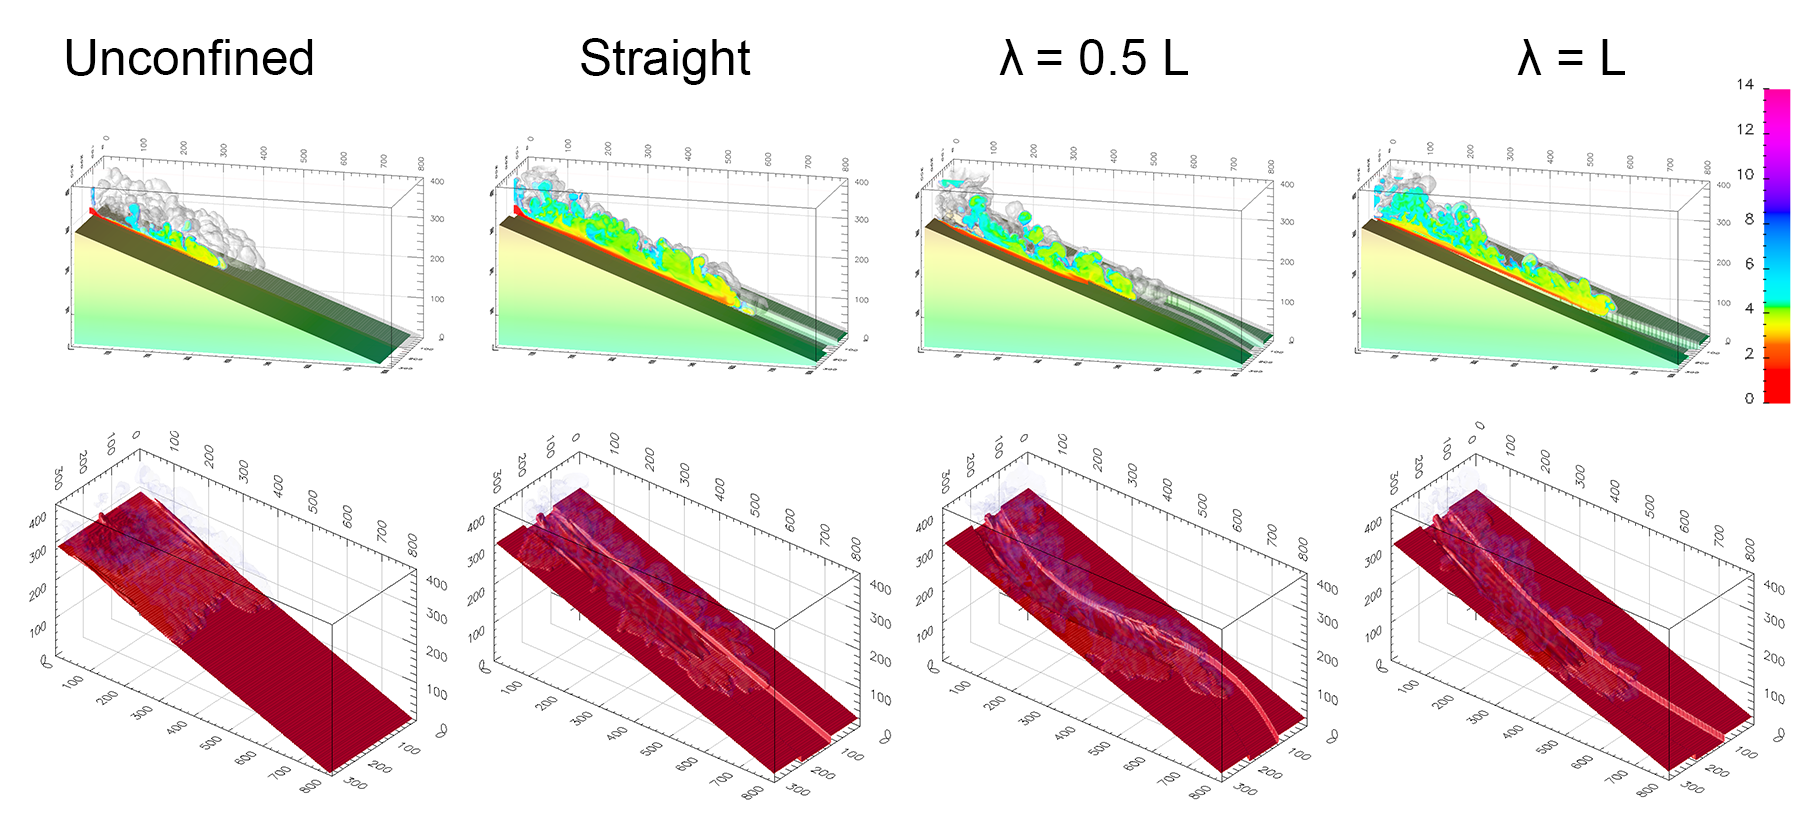
\includegraphics[width= \linewidth]{simulations_24.png}
 \caption{ Vertical profiles of volume fraction at L=0.2. Red colors show the dense limit at 2.5 volume fraction particles. While the blue outlines show the dilute limit of the current at 6.5 volume fraction particles. }
 \label{fig:sim} 
\end{figure}


\section{Discussion and Conclusion}
\label{sec:dis}
\subsection{Entrainment}
Profiles show the classic forms of pyroclastic density currents with high velocity noses at the head and a slightly less dense portion at the base of the flow where there is entrainment due to Lobe-Cleft instabilites (Dufek and Bergantz, 2007a; Dufek, 2016). The peak speed for all flows occurs in the first 10 m of the height and most flows significantly accelerated from the initial speed with the straight channel having the highest overall velocity. 

Temperature profiles in the flow show that the basal portions remain relatively hot while the dilute portions cool to close to ambient quickly. These thermal structures largely mirror the density profiles of the flow. The straight channel show higher velocities while the 800m channel shows a dense basal layer formation and the highest temperatures which remain largely unchanged from initial temperatures in this basal layer of the flow. This indicates less entrainment however bulk entrainment was higher than the straight channel. This indicates more entrainment at the dilute billows of the flow which is also seen in the higher overall height. This suggests possible decoupling due to slight bend of the channel of the dense and dilute portions which would shear the flow and increase entrainment in the dilute portions. 

\begin{figure}[ht]
 \centering
 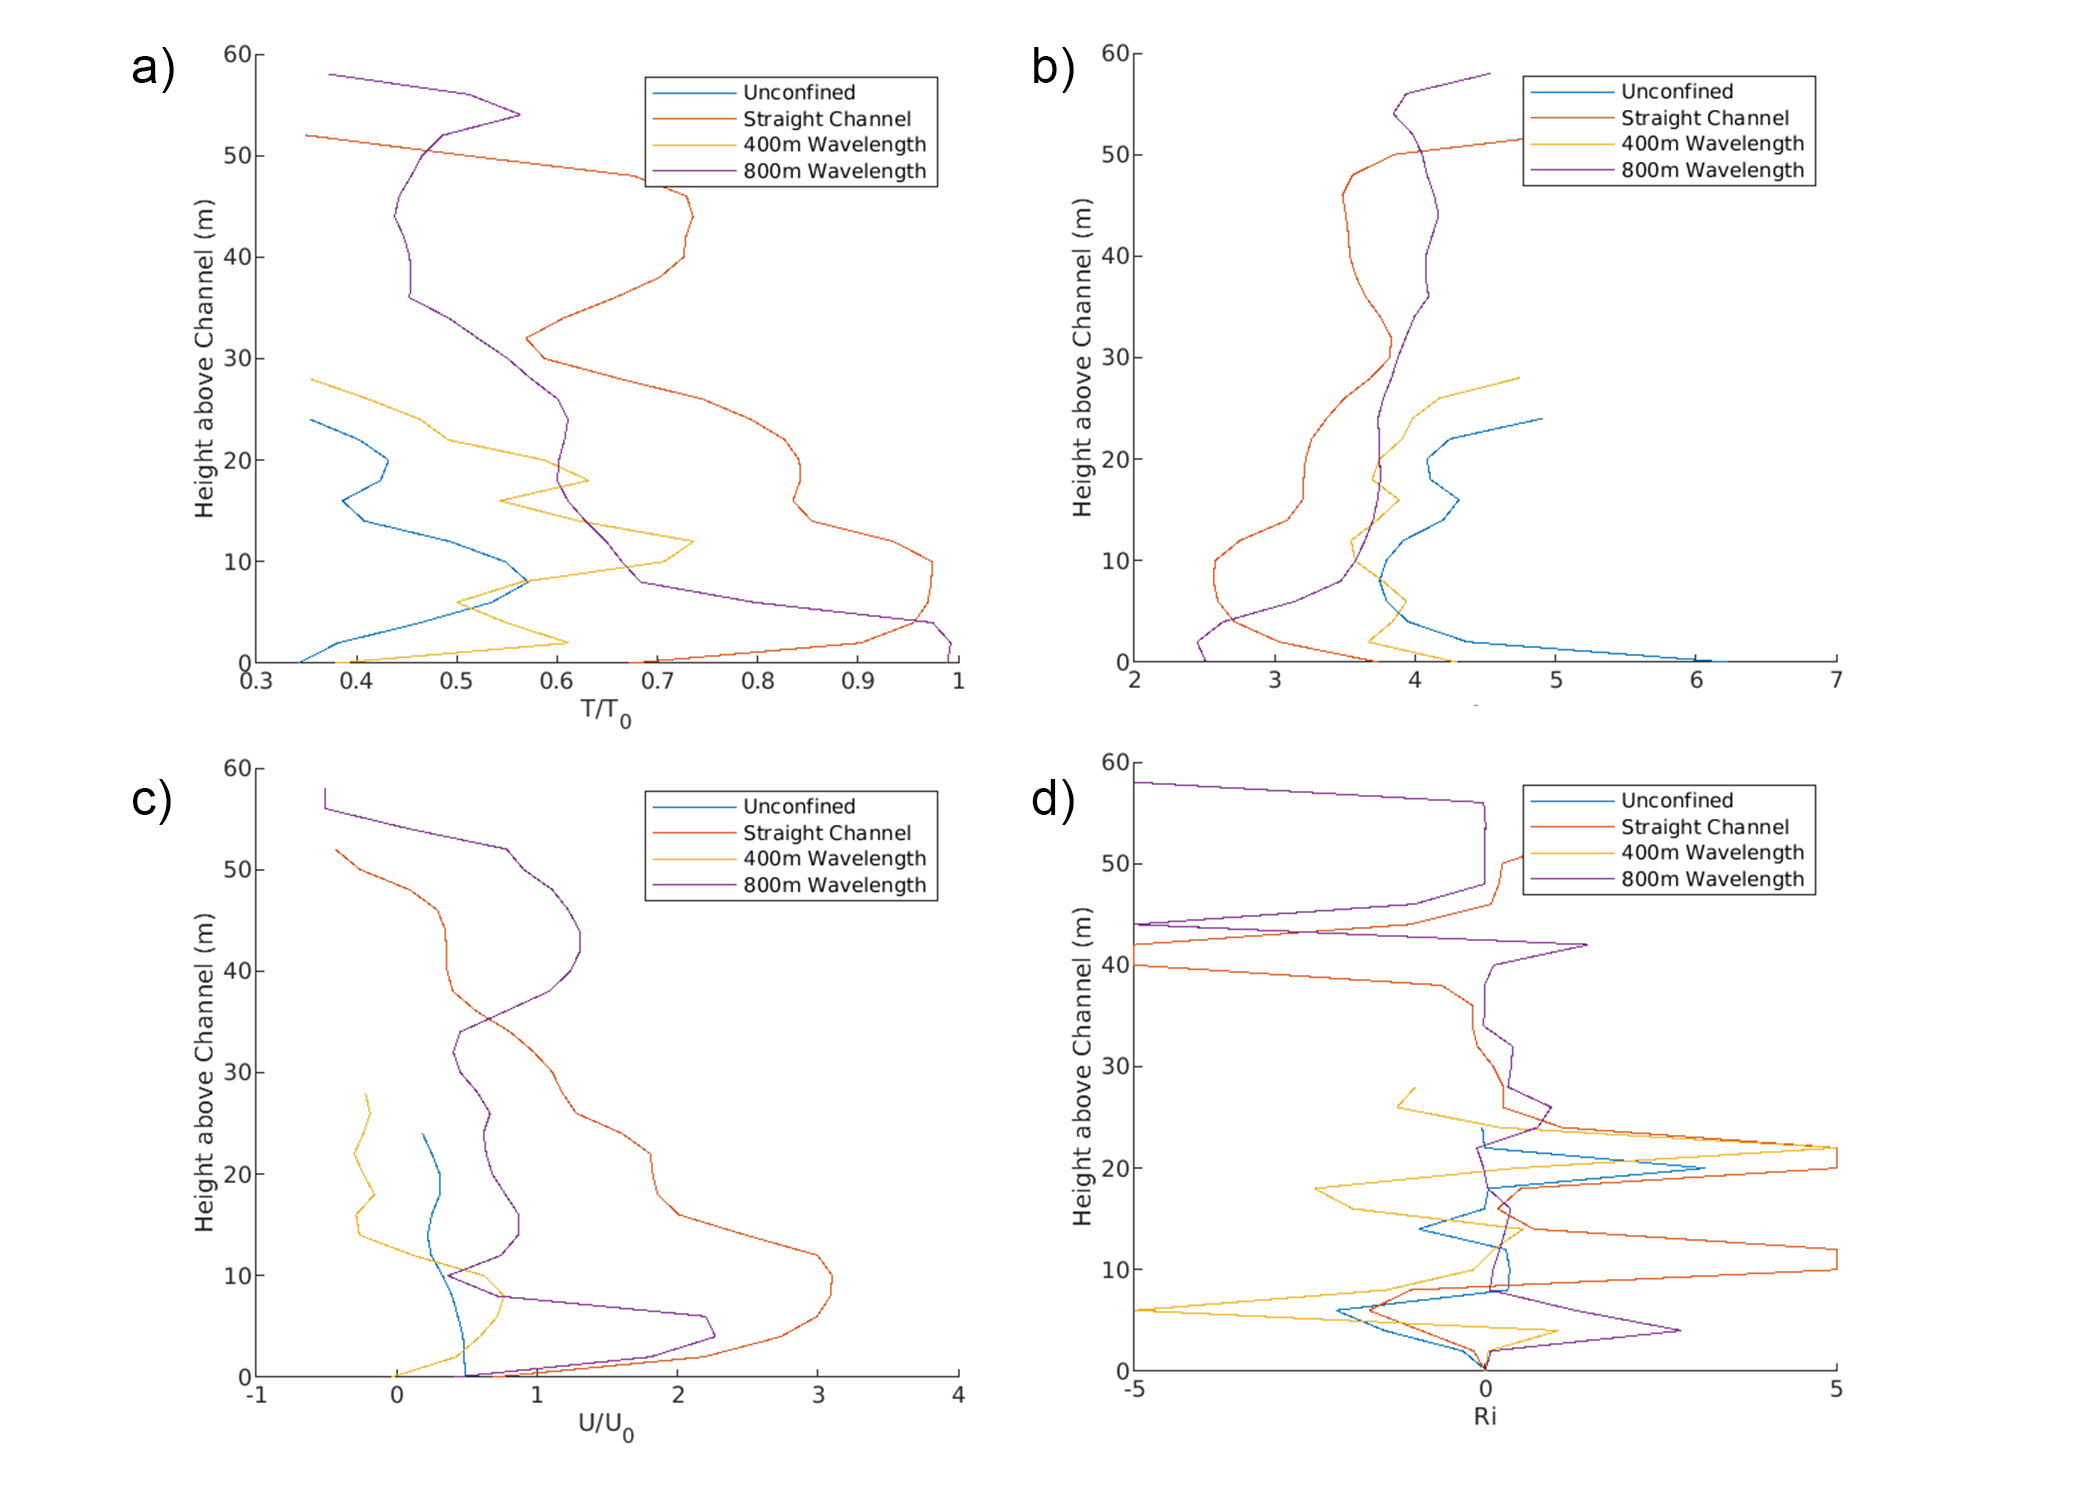
\includegraphics[width= \linewidth]{vertical.png}
 \caption{ Shows vertical profiles of PDCs at in the middle of the channel at L=0.5 t= 20 s.  \textbf{a)} Shows the vertical thermal profile for 4 simulations.  \textbf{b)} Vertical distribution of density \textbf{c)} vertical velocity profile.  \textbf{d)} Richardson number in the column (needs time averaging).}
 \label{fig:vert} 
\end{figure}
Channelization decreases entrainment for straight channels due to the decreased ability to form Lobe-Cleft instabilities which allows for denser basal layers to form ( I intend to look into this more by looking at the dense vs dilute entrainments). Channelization necessarily leads to decreased flow are which also correlates to decreased entrainment in both the dense and dilute portion. 

To explore entrainment and turbulence we use the Richardson number which a dimensionless number relating the density stratification to flow shear stress. Looking at Figure 4b. the large spikes in Richardson number shows a fully turbulent flow with greater turbulence in the channelized flows than the unconfined flow. This increase in turbulence may be associated with interaction with the channel sides or due to the faster velocities.

\subsection{Avulsion Mechanism}
\begin{figure}[ht]
 \centering
 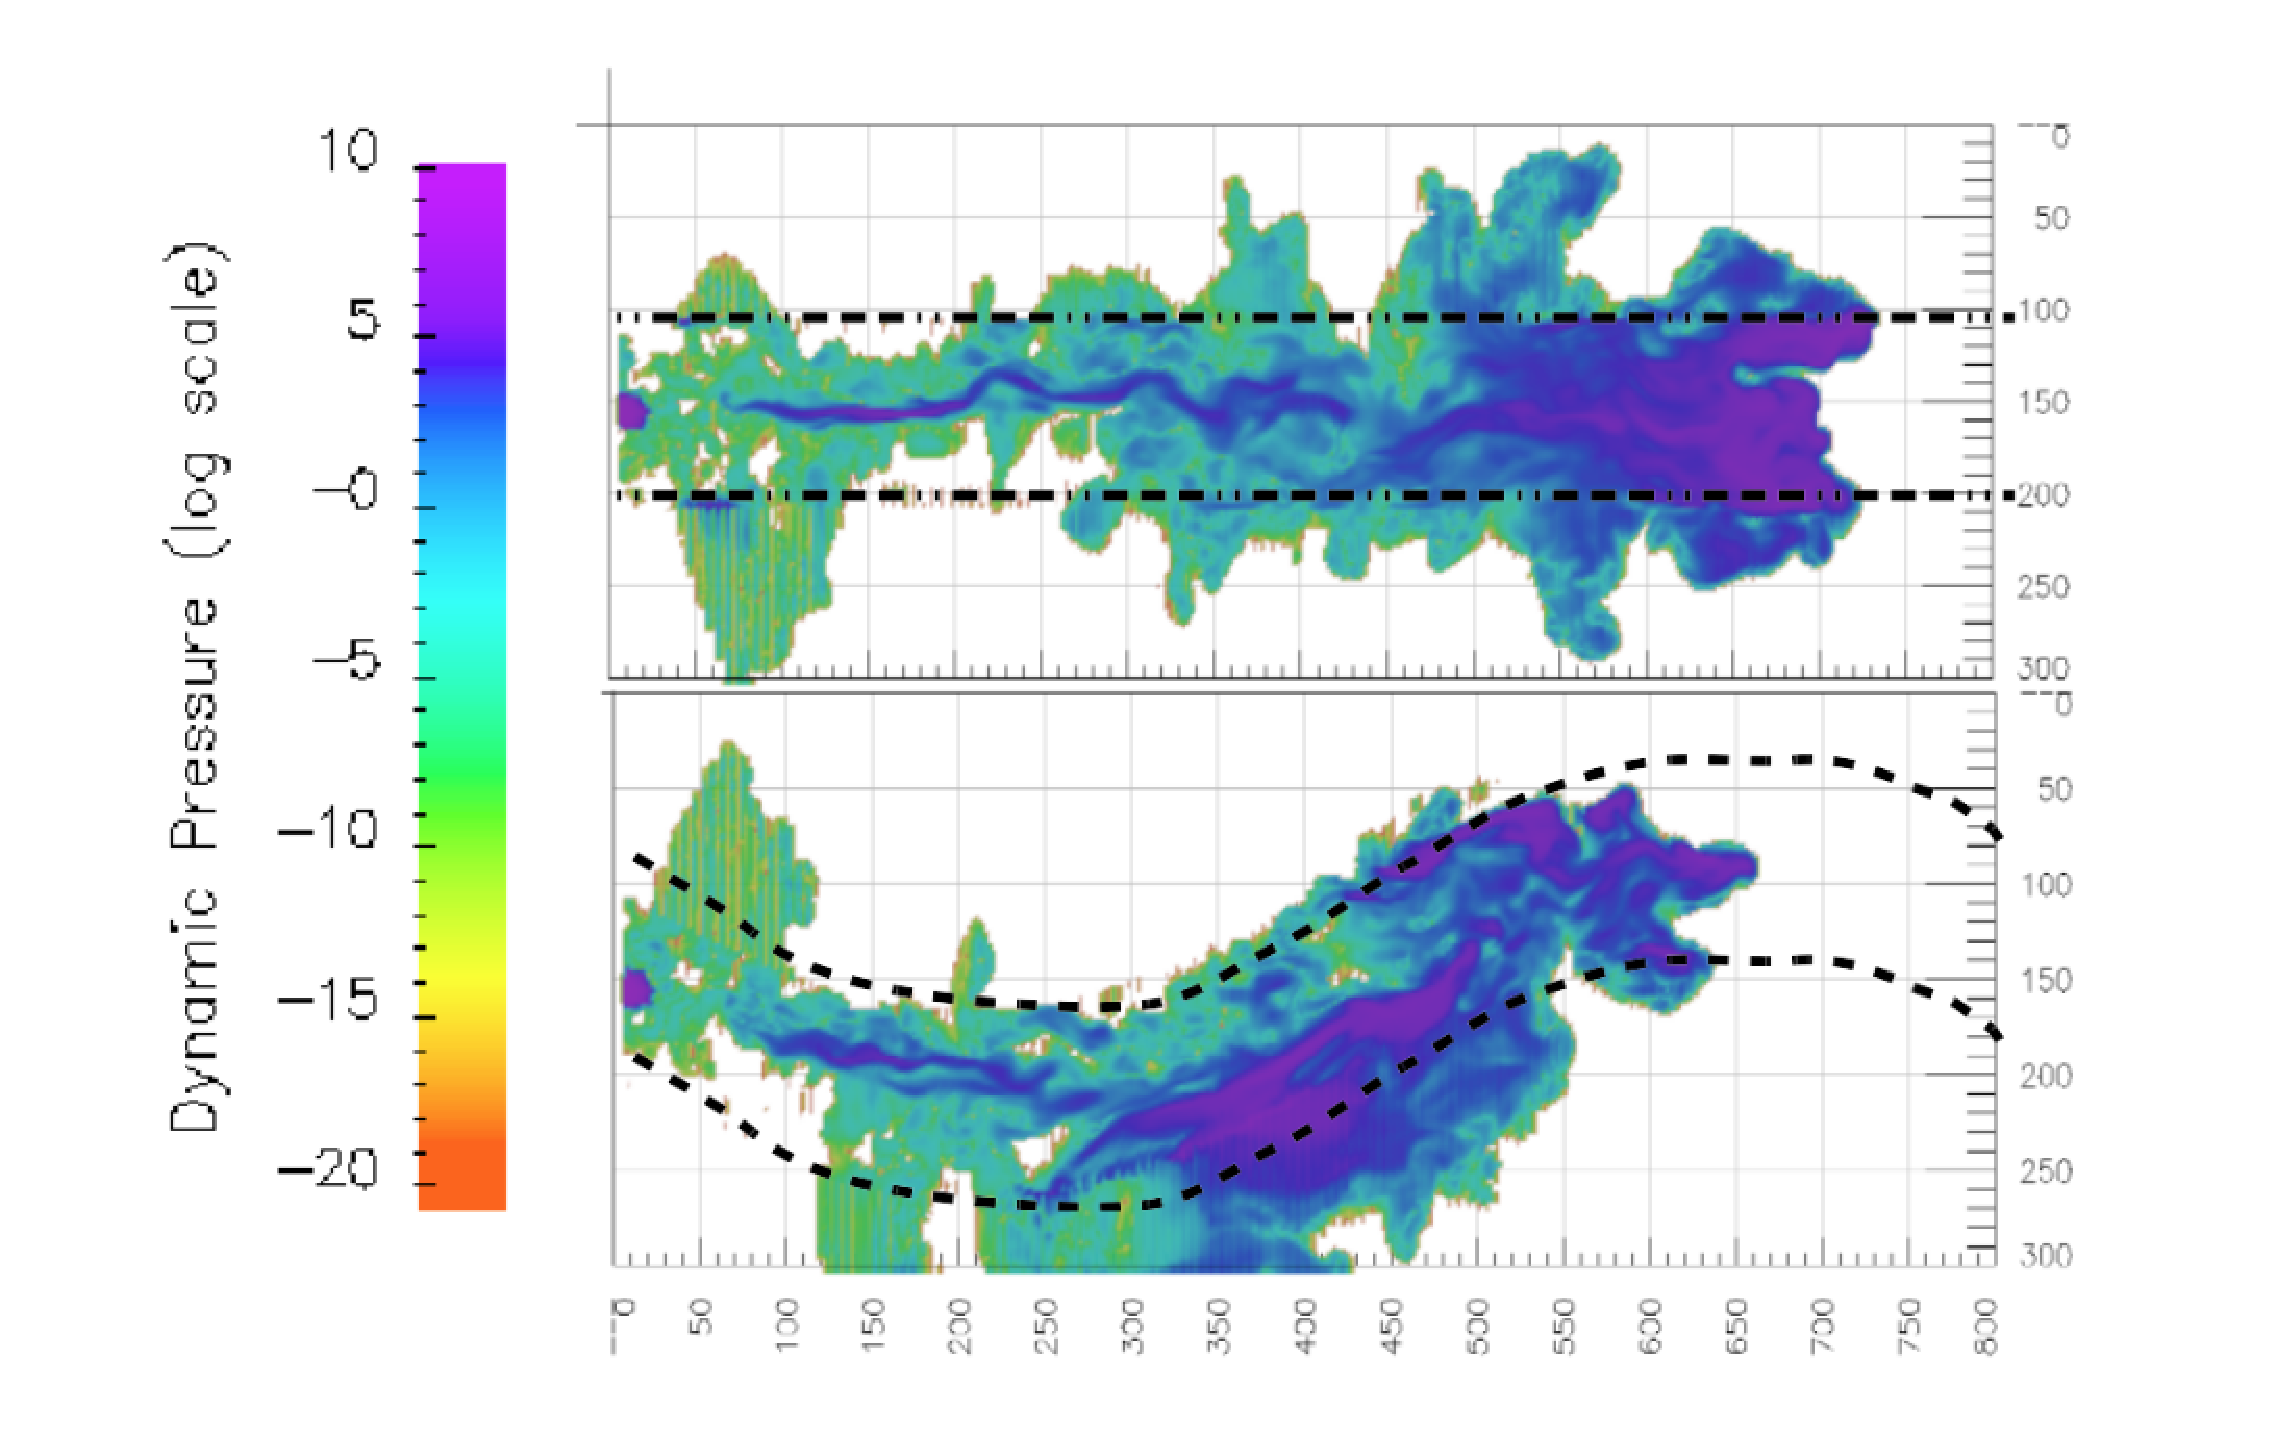
\includegraphics[width= \linewidth]{dpu.eps}
 \caption{ Shows dynamic pressure with the channel boundaries as a dashed line for the the straight (top) and sinuous cases (bottom). }
 \label{fig:dpu} 
\end{figure}
Our simulations show that the avulsion mechanism, in this case, is the overspill of the dense portion of the flow over the topography rather than decoupling of the dilute portions (although this is likely happening as well). To investigate this we consider the dynamic pressure:
\begin{equation}
    P_{d} = \frac{\rho u^{2}}{2}
\end{equation}
 where \(\rho\) is the mixture density and u is the velocity. In the sinuous flow, the dynamic pressure is greatest at the edge of the confining bend compared to the straight channel which shows the greatest dynamic pressure at the head of the flow. This indicates that at the bend the flow is both accelerating and compacting as it hits the wall of the channel. However even after the flow overwhelms the channel it stays at high dynamic pressure meaning there is little energy and density loss in the initial avulsion. This compaction allows for the passive overspill seen in Figure 6. This mechanism is consistent with field observations by Lube (2011) and Gertisser et al. (2013).



\begin{figure}[ht]
 \centering
 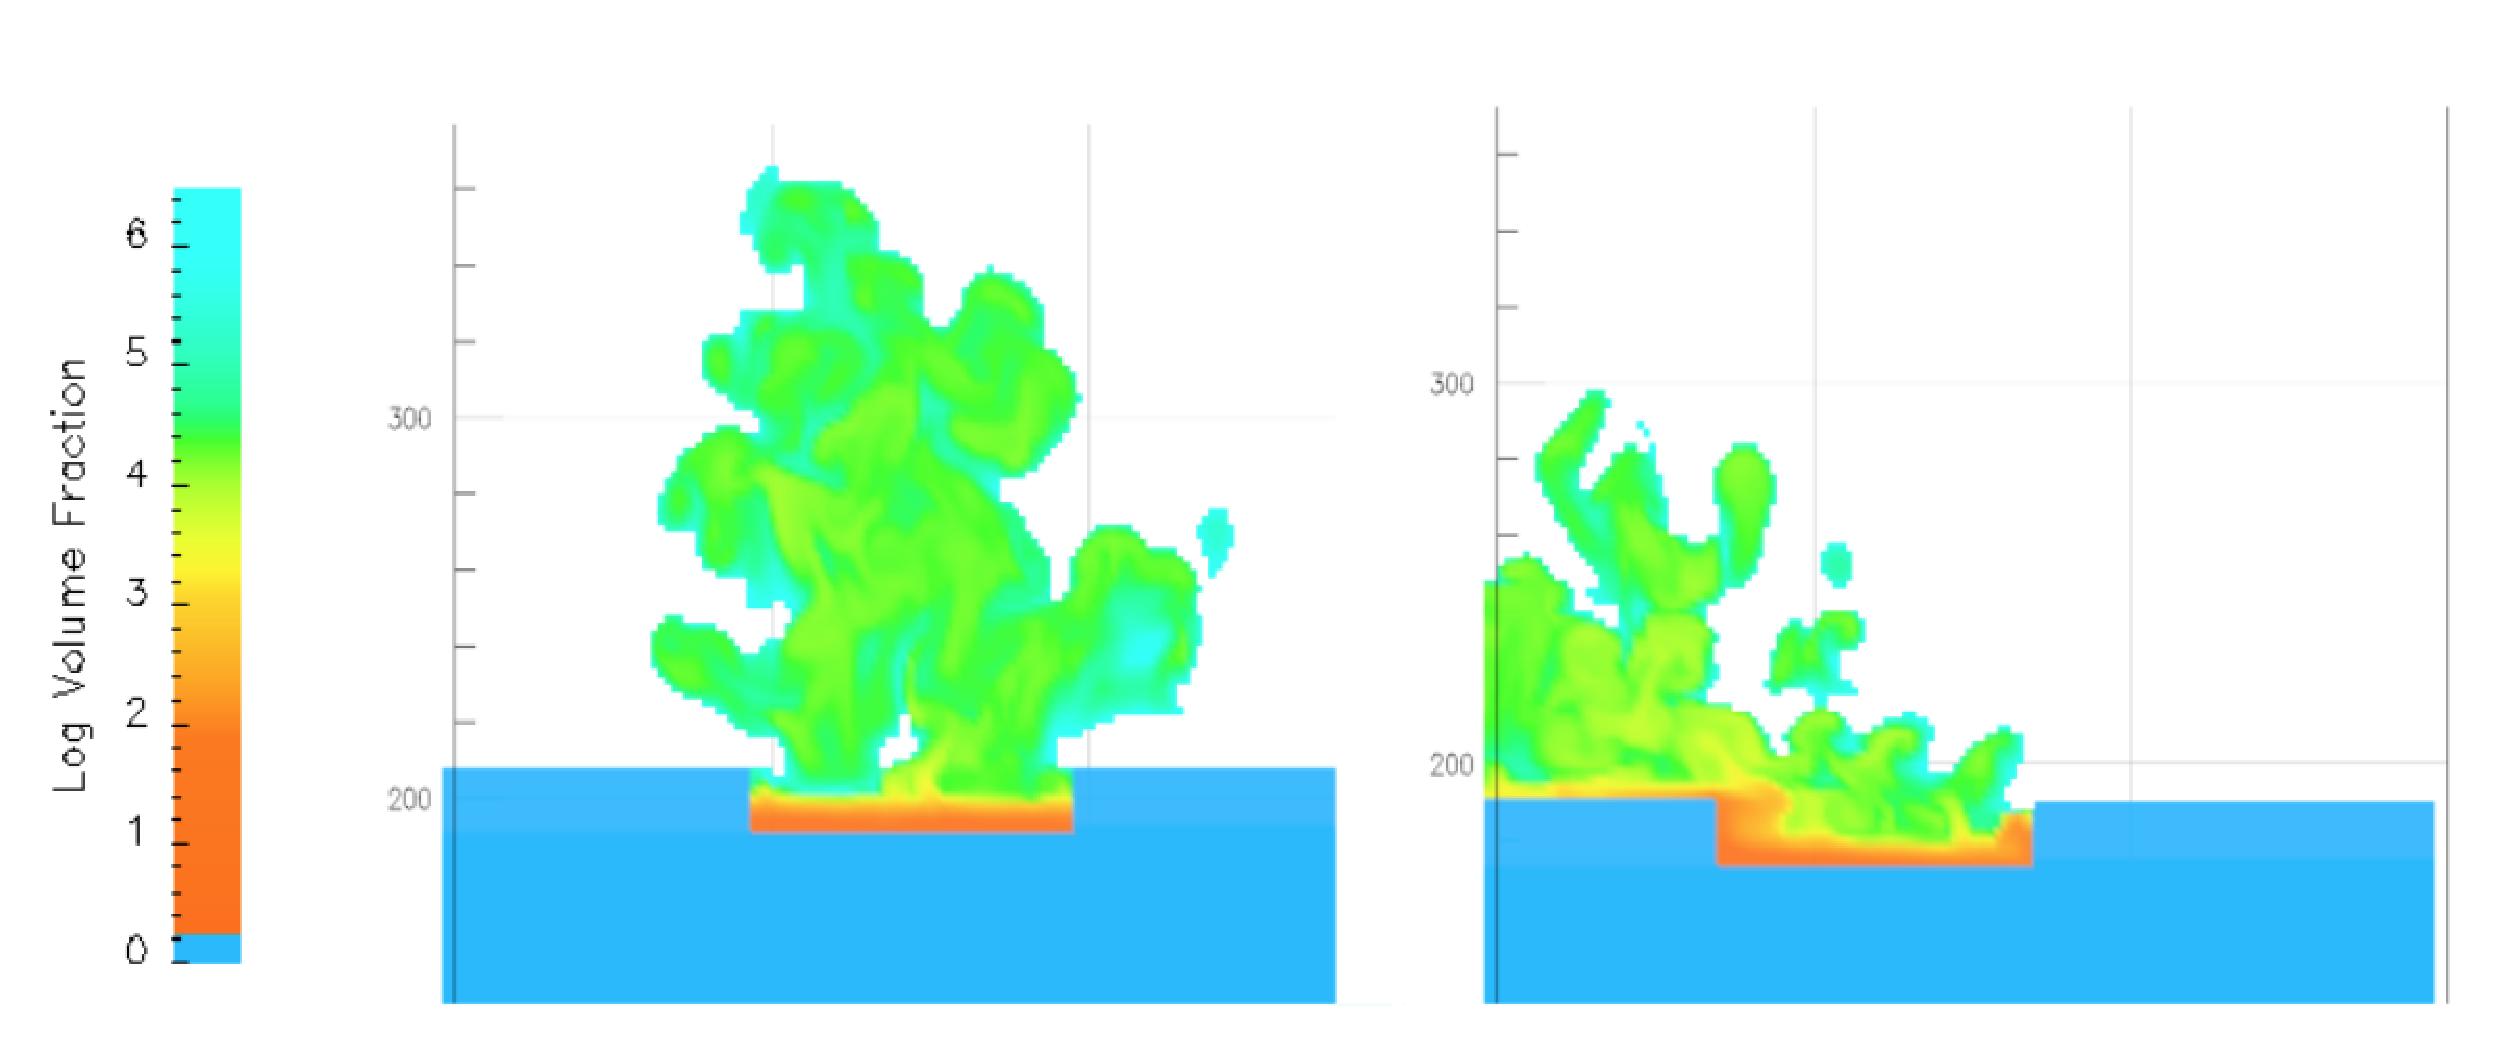
\includegraphics[width= \linewidth]{overspill.eps}
 \caption{ Vertical profiles of volume fraction at L=0.2. Red colors show denser portions of the flow. On the left is the straight channel case and on the right shows the sinuous channel case with avulsion. }
 \label{fig:ove} 
\end{figure}


\subsection{Conclusion}
Channelization does increases runout distances while decreasing entrainment relative to the unconfined case. This decrease in entrainment is due to the reduced flow area and ability to entrain air into the dense portions of the flow via Lobe-Cleft instabilities. Overspill occurs in the two sinuous channel simulations with more vigorous avulsion in the lower wavelength channels. This overspill is due to the passive overflow of the dense portion of the flow. 
Further work on this (that I will do for my next draft) includes expanding the parameter space of topography, constraining volume flux, time averaging vertical profiles, denser flows, and continued investigation into the avulsion mechanism. 


%%%%%%%%%%%%%%%%%%%%%%%%%%%%%%%%%%%%%%%%%%%%%%%%%%%%%%%%%%%%%%%%
%
%  ACKNOWLEDGMENTS

\acknowledgments
This work is supported by XXXX NSF grant XXX to JD. 
This work is supported by GLADE REU program, National Science Foundation Grant No. EAR-1255040. 
This work used the Extreme Science and Engineering Discovery Environment (XSEDE), which is supported by National Science Foundation Grant No. ACI-1053575.


%%  REFERENCE LIST AND TEXT CITATIONS
%
% Either type in your references using
%
% \begin{thebibliography}{}
% \bibitem{}
% Text
% \end{thebibliography}
%
% Or, to use BibTeX:
%
% Follow these steps
%
% 1. Type in \bibliography{<name of your .bib file>} 
%    Run LaTeX on your LaTeX file.
%
% 2. Run BiBTeX on your LaTeX file.
%
% 3. Open the new .bbl file containing the reference list and
%   copy all the contents into your LaTeX file here.
%
% 4. Run LaTeX on your new file which will produce the citations.
%
% AGU does not want a .bib or a .bbl file. Please copy in the contents of your .bbl file here.
\nocite{*}
\bibliography{channel.bib}

%%%%%%%%%%%%%%%%%%%%%%%%%%%%%%%%%%%%%%%%%
% Track Changes:
% To add words, \added{<word added>}
% To delete words, \deleted{<word deleted>}
% To replace words, \replace{<word to be replaced>}{<replacement word>}

% At the end of the document, use \listofchanges, which will list the
% changes and the page and line number where the change was made.

% When final version, \listofchanges will not produce anything,
% \added{} word will be printed, \deleted{} will take away the word,
% \replaced{}{} will print only the 2nd argument.

%%%

\end{document}

%%%%%%%%%%%%%%%%%%%%%%%%%%%%%%%%%%%%%
%% Supporting Information
%% (Optional) See AGUSuppInfoSamp.tex/pdf for requirements 
%% for Supporting Information.
%%%%%%%%%%%%%%%%%%%%%%%%%%%%%%%%%%%%%


%%%%%%%%%%%%%%%%%%%%%%%%%%%%%%%%%%%%%%%%%%%%%%%%%%%%%%%%%%%%%%%

More Information and Advice:

%% ------------------------------------------------------------------------ %%
%
%  SECTION HEADS
%
%% ------------------------------------------------------------------------ %%

% Capitalize the first letter of each word (except for
% prepositions, conjunctions, and articles that are
% three or fewer letters).

% AGU follows standard outline style; therefore, there cannot be a section 1 without
% a section 2, or a section 2.3.1 without a section 2.3.2.
% Please make sure your section numbers are balanced.
% ---------------
% Level 1 head
%
% Use the \section{} command to identify level 1 heads;
% type the appropriate head wording between the curly
% brackets, as shown below.
%
%An example:
%\section{Level 1 Head: Introduction}
%
% ---------------
% Level 2 head
%
% Use the \subsection{} command to identify level 2 heads.
%An example:
%\subsection{Level 2 Head}
%
% ---------------
% Level 3 head
%
% Use the \subsubsection{} command to identify level 3 heads
%An example:
%\subsubsection{Level 3 Head}
%
%---------------
% Level 4 head
%
% Use the \subsubsubsection{} command to identify level 3 heads
% An example:
%\subsubsubsection{Level 4 Head} An example.
%
%% ------------------------------------------------------------------------ %%
%
%  IN-TEXT LISTS
%
%% ------------------------------------------------------------------------ %%
%
% Do not use bulleted lists; enumerated lists are okay.
% \begin{enumerate}
% \item
% \item
% \item
% \end{enumerate}
%
%% ------------------------------------------------------------------------ %%
%
%  EQUATIONS
%
%% ------------------------------------------------------------------------ %%

% Single-line equations are centered.
% Equation arrays will appear left-aligned.

%Math coded inside display math mode \[ ...\]
% will not be numbered, e.g.,:
% \[ x^2=y^2 + z^2\]

 %Math coded inside \begin{equation} and \end{equation} will
 %be automatically numbered, e.g.,:
 %\begin{equation}
 %%x^2=y^2 + z^2
 %\end{equation}


% To create multiline equations, use the
% \begin{eqnarray} and \end{eqnarray} environment
% as demonstrated below.
%\begin{eqnarray}
%  x_{1} & = & (x - x_{0}) \cos \Theta \nonumber \\
%        && + (y - y_{0}) \sin \Theta  \nonumber \\
%  y_{1} & = & -(x - x_{0}) \sin \Theta \nonumber \\
%        && + (y - y_{0}) \cos \Theta.
%\end{eqnarray}

%If you don't want an equation number, use the star form:
%\begin{eqnarray*}...\end{eqnarray*}

% Break each line at a sign of operation
% (+, -, etc.) if possible, with the sign of operation
% on the new line.

% Indent second and subsequent lines to align with
% the first character following the equal sign on the
% first line.

% Use an \hspace{} command to insert horizontal space
% into your equation if necessary. Place an appropriate
% unit of measure between the curly braces, e.g.
% \hspace{1in}; you may have to experiment to achieve
% the correct amount of space.


%% ------------------------------------------------------------------------ %%
%
%  EQUATION NUMBERING: COUNTER
%
%% ------------------------------------------------------------------------ %%

% You may change equation numbering by resetting
% the equation counter or by explicitly numbering
% an equation.

% To explicitly number an equation, type \eqnum{}
% (with the desired number between the brackets)
% after the \begin{equation} or \begin{eqnarray}
% command.  The \eqnum{} command will affect only
% the equation it appears with; LaTeX will number
% any equations appearing later in the manuscript
% according to the equation counter.
%

% If you have a multiline equation that needs only
% one equation number, use a \nonumber command in
% front of the double backslashes (\\) as shown in
% the multiline equation above.

% If you are using line numbers, remember to surround
% equations with \begin{linenomath*}...\end{linenomath*}

%  To add line numbers to lines in equations:
%  \begin{linenomath*}
%  \begin{equation}
%  \end{equation}
%  \end{linenomath*}



